\documentclass[12pt,a4paper]{article}
\usepackage{amsmath,amsthm,amssymb,mathtools}
\usepackage{tikz}
\usetikzlibrary{arrows.meta,positioning,shapes.geometric,calc,fit,backgrounds}
\usepackage{graphicx}
\usepackage{booktabs,tabularx,multirow}
\usepackage[ruled,vlined,linesnumbered]{algorithm2e}
\usepackage[most]{tcolorbox}
\usepackage{hyperref}
\usepackage[capitalize,noabbrev]{cleveref}
\usepackage[margin=1in]{geometry}
\usepackage{fancyhdr}
\usepackage{enumitem}
\usepackage{xcolor}

%% ------------------------------------------------------------------
%%  tcolorbox environments
%% ------------------------------------------------------------------
\newtcolorbox{keyinsight}[1][]{colback=blue!5!white,colframe=blue!75!black,fonttitle=\bfseries,title=Key Insight,#1}
\newtcolorbox{example}[1][]{colback=green!5!white,colframe=green!75!black,fonttitle=\bfseries,title=Example,#1}
\newtcolorbox{warningbox}[1][]{colback=red!5!white,colframe=red!75!black,fonttitle=\bfseries,title=Warning,#1}

%% ------------------------------------------------------------------
%%  amsthm environments
%% ------------------------------------------------------------------
\newtheorem{theorem}{Theorem}[section]
\newtheorem{lemma}[theorem]{Lemma}
\newtheorem{definition}{Definition}[section]
\newtheorem{remark}{Remark}[section]

%% ------------------------------------------------------------------
%%  Header / footer
%% ------------------------------------------------------------------
\pagestyle{fancy}
\fancyhf{}
\rhead{Deep Learning --- Session 24}
\lhead{Attention Mechanism \& Transformer Motivation}
\cfoot{\thepage}
\renewcommand{\headrulewidth}{0.4pt}

%% ------------------------------------------------------------------
%%  Convenience macros
%% ------------------------------------------------------------------
\newcommand{\ct}{c_t}
\newcommand{\hi}{h_i}
\newcommand{\hj}{h_j}
\newcommand{\st}{s_t}
\newcommand{\eij}{e_{ij}}
\newcommand{\aij}{\alpha_{ij}}

%% ------------------------------------------------------------------
\begin{document}

%% ==================================================================
%%  TITLE PAGE
%% ==================================================================
\begin{titlepage}
  \centering
  \vspace*{2cm}
  {\LARGE\bfseries Deep Learning Course\par}
  \vspace{0.5cm}
  {\large Indian Institute of Information Technology Dharwad\par}
  \vspace{1.5cm}
  \rule{\linewidth}{0.5mm}\\[0.4cm]
  {\huge\bfseries Session 24\par}
  \vspace{0.3cm}
  {\Large\bfseries Attention Mechanism and Transformer Motivation\par}
  \rule{\linewidth}{0.5mm}\\[1.5cm]

  \begin{tabular}{rl}
    \textbf{Instructors:}  & Prof.\ S R M Prasanna \& Dr.\ Sunil Saumya \\[4pt]
    \textbf{Date:}         & February 14, 2026                           \\[4pt]
    \textbf{Lecture Deck:} & \texttt{10-Seq2Seq} (slides 24--36 / 37)    \\[4pt]
    \textbf{Duration:}     & $\approx 1$ hour 47 minutes                 \\[4pt]
    \textbf{Video:}        & \url{https://vimeo.com/1164910639}          \\
  \end{tabular}

  \vfill
  {\large\itshape
    ``Not all inputs are equally important ---
    Attention teaches the decoder where to look.''\par}
  \vspace{1cm}
  {\normalsize Lecture notes compiled from video transcript and slide
    visual extractions.\par}
\end{titlepage}

%% ==================================================================
%%  TABLE OF CONTENTS
%% ==================================================================
\tableofcontents
\newpage

%% ==================================================================
\section{Introduction}
\label{sec:intro}
%% ==================================================================

Session~24 marks the transition from vanilla Sequence-to-Sequence
(Seq2Seq) modelling to the \textbf{Attention mechanism}, the
conceptual precursor of every modern large language model.  The
session opens by revisiting the bottleneck that motivated attention,
builds up the mechanics step by step through a concrete Hindi
machine-translation example, derives the full Bahdanau (additive)
attention formulation, contrasts it with Luong (multiplicative)
attention, and closes by showing why even the best attention-equipped
LSTM system cannot escape the fundamental sequential bottleneck ---
the insight that gave birth to the \textbf{Transformer} in 2017.

\subsection*{Session Objectives}
\begin{enumerate}[label=\arabic*.]
  \item Understand why the fixed context vector of vanilla Seq2Seq
        is a performance bottleneck.
  \item Formalise the notion of a \emph{dynamic} context vector
        $\ct$ that changes at every decoder time step.
  \item Derive the Bahdanau attention alignment score, softmax
        normalisation, and context vector computation.
  \item Compare Bahdanau (additive) and Luong (multiplicative)
        attention.
  \item Identify the remaining O$(n^{2})$ complexity and sequential
        bottleneck that motivates the Transformer architecture.
\end{enumerate}

\begin{keyinsight}[title=Session Theme]
  The central insight of attention is that \emph{not all encoder
  hidden states are equally relevant} to every decoder step.
  Attention learns a probability distribution over encoder states
  dynamically, giving each decoder step a tailored context vector
  rather than a single fixed one.
\end{keyinsight}

%% ==================================================================
\section{Background and Prerequisites}
\label{sec:background}
%% ==================================================================

\subsection{Sequence-to-Sequence Recap}

A Sequence-to-Sequence (Seq2Seq) model \cite{sutskever2014} consists
of two LSTM networks:

\begin{itemize}
  \item \textbf{Encoder}: reads the entire input sequence
        $x_1, x_2, \ldots, x_n$ one token at a time and produces a
        fixed-dimensional \emph{context vector} $C$ from its final
        hidden state $h_n$.
  \item \textbf{Decoder}: starting from $C$ (used as the initial
        hidden state $s_{-1}$), generates the output sequence
        $y_1, y_2, \ldots, y_m$ autoregressively --- each token is
        predicted conditioned on all previously generated tokens and
        on the same fixed $C$.
\end{itemize}

\begin{definition}[Context Vector --- Vanilla Seq2Seq]
\label{def:ctx-vanilla}
In standard Seq2Seq the context vector is
\begin{equation}
  C = h_n,
  \label{eq:ctx-vanilla}
\end{equation}
where $h_n \in \mathbb{R}^{d}$ is the final encoder hidden state
and $d$ is the hidden dimension.  $C$ is \emph{identical} at every
decoder time step.
\end{definition}

\subsection{Why Variable-Length Sequences Require Seq2Seq}

Standard single-stack RNN / LSTM architectures require the input and
output sequences to be the same length.  Machine translation breaks
this assumption: ``I am going'' (3 tokens) maps to
``\foreignlanguage{hindi}{main ja raha hoon}'' (4 tokens in Hindi).
Seq2Seq decouples the encoder and decoder, allowing arbitrary input
and output lengths.

\subsection{The Fixed-Context Bottleneck}

Although Seq2Seq solved the variable-length problem, compressing an
arbitrarily long input into a single fixed vector $C$ creates two
compounding problems:

\begin{enumerate}[label=(\alph*)]
  \item \textbf{Information loss}: LSTM gates must selectively forget
        information as the sequence grows; very early tokens may be
        under-represented in $h_n$.
  \item \textbf{Uniform relevance}: the decoder receives the same
        $C$ at every step even though the relevant source tokens
        change.  When generating the Hindi word for ``I'', the source
        word ``I'' is most relevant; when generating the word for
        ``going'', the source word ``going'' dominates.  A single
        vector cannot express both biases simultaneously.
\end{enumerate}

\begin{warningbox}
  Empirically, vanilla Seq2Seq BLEU score drops sharply for sentence
  lengths beyond 20 tokens.  The fixed context vector cannot
  faithfully encode long-range dependencies, resulting in inaccurate
  translations.
\end{warningbox}

%% ==================================================================
\section{Attention Intuition}
\label{sec:intuition}
%% ==================================================================

\subsection{Cognitive Motivation}

The attention mechanism is inspired by how the human brain processes
information.  When scanning a page of text for a specific word (e.g.\
\texttt{PASSWORD} hidden in a wall of filler words), the brain does
not process every word with equal effort; it \emph{focuses} on the
salient signal and ignores the noise.

\cref{fig:attention-intuition} illustrates this idea.

\begin{figure}[ht]
\centering
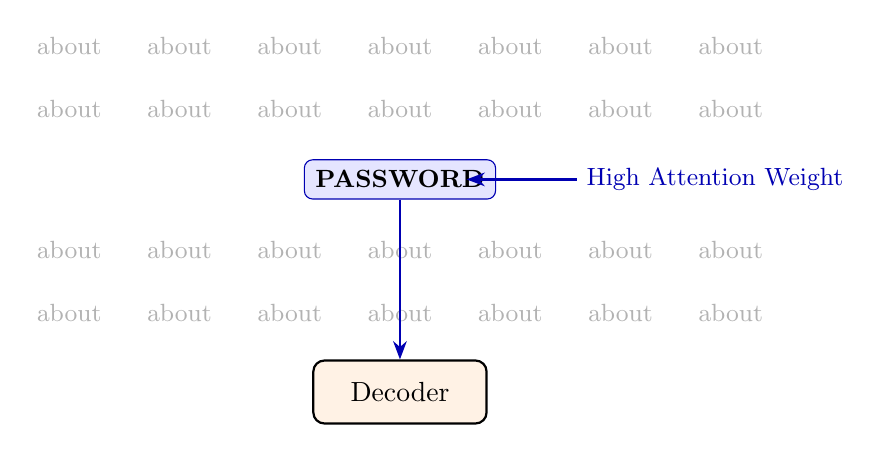
\begin{tikzpicture}[
    word/.style={font=\small, text=gray!60},
    highlight/.style={draw=blue!70!black, fill=blue!10,
                      rounded corners=3pt, inner sep=4pt,
                      font=\small\bfseries},
    arr/.style={-{Stealth}, thick, blue!70!black}
  ]
  % Background noise words
  \foreach \x in {0,1.4,2.8,4.2,5.6,7.0,8.4} {
    \node[word] at (\x, 3.2)  {about};
    \node[word] at (\x, 2.4)  {about};
    \node[word] at (\x, 0.6)  {about};
    \node[word] at (\x, -0.2) {about};
  }
  % Highlighted word
  \node[highlight] (pw) at (4.2, 1.5) {PASSWORD};
  % Arrow annotation
  \node[font=\small, text=blue!70!black] (ann) at (8.2, 1.5)
        {High Attention Weight};
  \draw[arr] (ann.west) -- +(-1.4,0);
  % Decoder box
  \node[draw, thick, fill=orange!10, rounded corners=4pt,
        minimum width=2.2cm, minimum height=0.8cm] (dec) at (4.2,-1.2)
        {Decoder};
  \draw[arr] (pw.south) -- (dec.north);
\end{tikzpicture}
\caption{Attention intuition: the salient word \texttt{PASSWORD}
         receives a high attention weight; filler words receive
         near-zero weight.  The decoder attends primarily to the
         relevant signal.}
\label{fig:attention-intuition}
\end{figure}

\begin{keyinsight}[title=Attention as Selective Focus]
  Neural attention formalises the cognitive notion of focus:
  at each decoder time step $t$, a learned scoring function assigns
  a scalar \emph{relevance} score to every encoder hidden state.
  After softmax normalisation, these scores form a probability
  distribution (the attention weights) that acts as a soft pointer
  into the encoder sequence.
\end{keyinsight}

\subsection{The Core Idea in One Sentence}

At every decoder time step $t$, instead of reading the same fixed
$C$, the model dynamically computes a \emph{weighted sum} of all
encoder hidden states, where the weights express how relevant each
source position is to the current generation step.

%% ==================================================================
\section{What Changes with Attention}
\label{sec:what-changes}
%% ==================================================================

\subsection{Structural Comparison}

\cref{tab:comparison} summarises the input to each decoder LSTM cell
in the two architectures.

\begin{table}[ht]
\centering
\caption{Standard Seq2Seq vs.\ Attention-augmented Seq2Seq: inputs
         to the decoder LSTM at each time step.}
\label{tab:comparison}
\begin{tabular}{@{}clll@{}}
\toprule
\textbf{Step} & \textbf{Standard Seq2Seq} & \textbf{With Attention} & \textbf{Difference} \\
\midrule
Step 0 & $(y_0,\; s_{-1})$      & $(y_0,\; s_{-1},\; c_0)$ & $c_0$ added \\
Step 1 & $(y_1,\; s_0)$         & $(y_1,\; s_0,\;   c_1)$  & $c_1$ added \\
Step 2 & $(y_2,\; s_1)$         & $(y_2,\; s_1,\;   c_2)$  & $c_2$ added \\
Step $t$ & $(y_t,\; s_{t-1})$   & $(y_t,\; s_{t-1},\; c_t)$ & $c_t$ added \\
\bottomrule
\end{tabular}
\end{table}

The key observation: in standard Seq2Seq $s_{-1} = C$ is the same
for every step and then changes only through the LSTM dynamics.  With
attention, an \emph{explicit} dynamic context vector $c_t$ is
computed fresh at each step, directly from all encoder hidden states.

\subsection{Architecture Diagram}

\cref{fig:arch-comparison} shows the architectural difference.

\begin{figure}[ht]
\centering
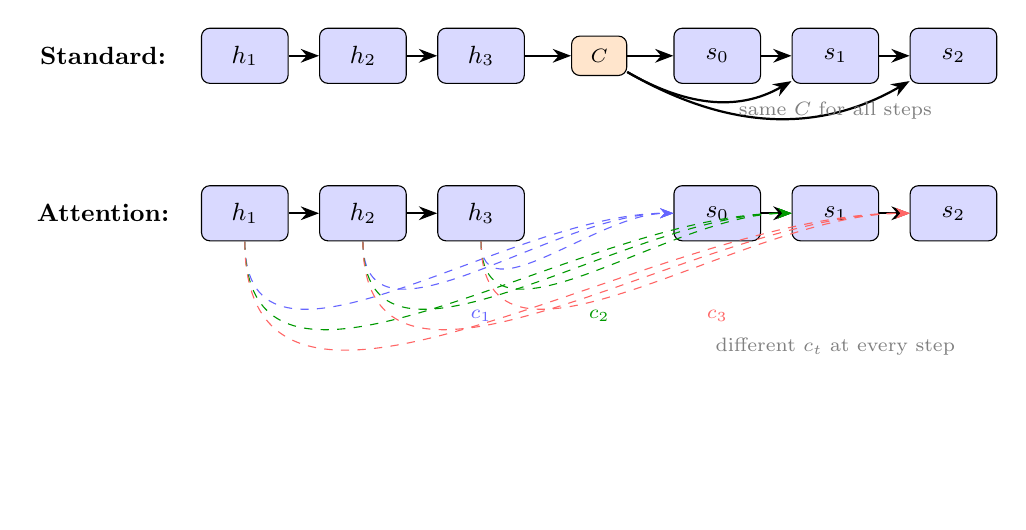
\begin{tikzpicture}[
    lstm/.style={draw, fill=blue!15, rounded corners=3pt,
                 minimum width=1.1cm, minimum height=0.7cm,
                 font=\small},
    ctx/.style={draw, fill=orange!20, rounded corners=3pt,
                minimum width=0.7cm, minimum height=0.5cm,
                font=\scriptsize},
    arr/.style={-{Stealth}, thick},
    labl/.style={font=\small\bfseries}
  ]
  %% --- Standard (top row) ---
  \node[labl] at (-1.8, 2.6) {Standard:};
  % Encoder LSTMs
  \node[lstm] (e1s) at (0,   2.6) {$h_1$};
  \node[lstm] (e2s) at (1.5, 2.6) {$h_2$};
  \node[lstm] (e3s) at (3.0, 2.6) {$h_3$};
  % Context
  \node[ctx]  (cs)  at (4.5, 2.6) {$C$};
  % Decoder LSTMs
  \node[lstm] (d1s) at (6.0, 2.6) {$s_0$};
  \node[lstm] (d2s) at (7.5, 2.6) {$s_1$};
  \node[lstm] (d3s) at (9.0, 2.6) {$s_2$};
  % Connections encoder
  \draw[arr] (e1s) -- (e2s);
  \draw[arr] (e2s) -- (e3s);
  \draw[arr] (e3s) -- (cs);
  % C to all decoder steps
  \draw[arr] (cs)  -- (d1s);
  \draw[arr] (cs)  to[out=-30,in=210] (d2s);
  \draw[arr] (cs)  to[out=-30,in=210] (d3s);
  \draw[arr] (d1s) -- (d2s);
  \draw[arr] (d2s) -- (d3s);
  \node[font=\scriptsize, text=gray] at (7.5, 1.9) {same $C$ for all steps};

  %% --- Attention (bottom row) ---
  \node[labl] at (-1.8, 0.6) {Attention:};
  % Encoder LSTMs
  \node[lstm] (e1a) at (0,   0.6) {$h_1$};
  \node[lstm] (e2a) at (1.5, 0.6) {$h_2$};
  \node[lstm] (e3a) at (3.0, 0.6) {$h_3$};
  % Decoder LSTMs
  \node[lstm] (d1a) at (6.0, 0.6) {$s_0$};
  \node[lstm] (d2a) at (7.5, 0.6) {$s_1$};
  \node[lstm] (d3a) at (9.0, 0.6) {$s_2$};
  % Encoder chain
  \draw[arr] (e1a) -- (e2a);
  \draw[arr] (e2a) -- (e3a);
  % Decoder chain
  \draw[arr] (d1a) -- (d2a);
  \draw[arr] (d2a) -- (d3a);
  % Attention arrows from all encoder to each decoder step
  \foreach \ea in {e1a,e2a,e3a} {
    \draw[-{Stealth}, dashed, blue!60] (\ea) to[out=270,in=180] (d1a);
    \draw[-{Stealth}, dashed, green!60!black] (\ea) to[out=270,in=180] (d2a);
    \draw[-{Stealth}, dashed, red!60] (\ea) to[out=270,in=180] (d3a);
  }
  \node[font=\scriptsize, text=blue!60]       at (3.0,-0.7) {$c_1$};
  \node[font=\scriptsize, text=green!60!black] at (4.5,-0.7) {$c_2$};
  \node[font=\scriptsize, text=red!60]         at (6.0,-0.7) {$c_3$};
  \node[font=\scriptsize, text=gray] at (7.5,-1.1)
        {different $c_t$ at every step};
\end{tikzpicture}
\caption{Architectural comparison.  \textit{Top:} Standard Seq2Seq
         passes the same context vector $C$ to every decoder step.
         \textit{Bottom:} Attention-augmented Seq2Seq computes a
         fresh $c_t$ at each decoder step as a weighted sum of all
         encoder hidden states $h_1, h_2, h_3$.}
\label{fig:arch-comparison}
\end{figure}

\begin{definition}[Dynamic Context Vector]
\label{def:dyn-ctx}
In an attention-augmented Seq2Seq model, the context vector at
decoder step $t$ is
\begin{equation}
  c_t = \sum_{i=1}^{T_{\mathrm{enc}}} \alpha_{ti}\, h_i,
  \label{eq:ctx-dynamic}
\end{equation}
where $T_{\mathrm{enc}}$ is the encoder sequence length,
$h_i \in \mathbb{R}^{d}$ is the encoder hidden state at position $i$,
and $\alpha_{ti} \geq 0$ are the \emph{attention weights} satisfying
$\sum_i \alpha_{ti} = 1$.
\end{definition}

\begin{keyinsight}[title=Dimensionality of $c_t$]
  The context vector $c_t$ is a \emph{vector}, not a scalar.  Its
  dimension equals the encoder hidden dimension $d$, because it is a
  weighted sum of $d$-dimensional encoder hidden states $h_i$.
  Each element of $c_t$ is the weighted average of the corresponding
  element across all $h_i$ vectors.
\end{keyinsight}

%% ==================================================================
\section{Attention Calculation: Step-by-Step Derivation}
\label{sec:calc}
%% ==================================================================

\subsection{Running Example}

Throughout this section we use the English-to-Hindi translation:

\begin{center}
  \textbf{Input (English):} \quad ``I'', ``am'', ``going'' \\[4pt]
  \textbf{Output (Hindi):}  \quad ``\textit{main}'', ``\textit{ja}'',
                                    ``\textit{raha}'', ``\textit{hoon}''
\end{center}

The encoder produces hidden states $h_1$ (for ``I''), $h_2$ (for
``am''), and $h_3$ (for ``going'').  Note that the sequences have
different lengths ($n=3$ vs.\ $m=4$), and the word order differs:
the verb ``going'' appears third in English but maps to both
\textit{ja} (position 2) and \textit{raha} (position 3) in Hindi.

\subsection{Attention at Decoder Step $t=1$}
\label{subsec:attn-t1}

At decoder step $t=1$ (generating the second Hindi word), the inputs
to the decoder LSTM are $y_1$ (the previously generated word
\textit{main}), $s_0$ (the decoder state after step 0), and the
newly computed context vector $c_1$.

The context vector is:
\begin{equation}
  c_1 = \alpha_{11}\,h_1 + \alpha_{12}\,h_2 + \alpha_{13}\,h_3,
  \label{eq:ctx-t1}
\end{equation}
where we expect $\alpha_{12}$ and $\alpha_{13}$ to be larger than
$\alpha_{11}$ because the Hindi word \textit{ja} (``go'') is
semantically aligned with the English word ``going'', not with ``I''.

\cref{fig:attention-calc} shows the full computation graph.

\begin{figure}[ht]
\centering
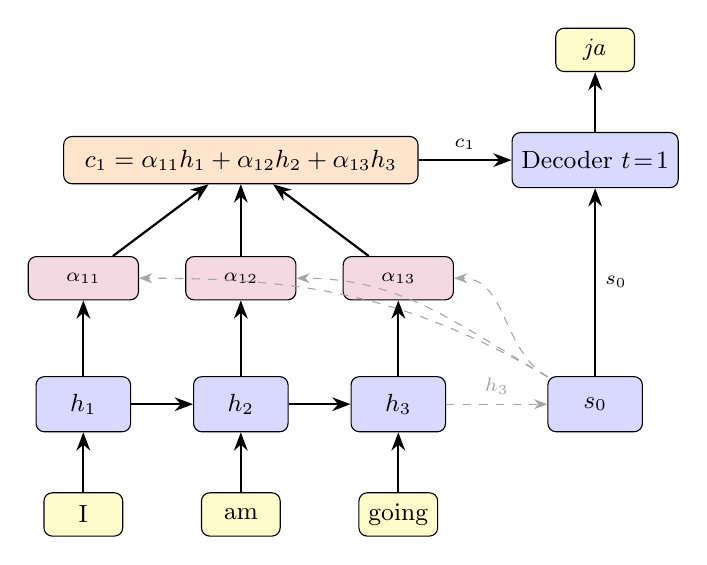
\begin{tikzpicture}[
    word/.style={draw, fill=yellow!20, rounded corners=3pt,
                 minimum width=1.0cm, minimum height=0.55cm,
                 font=\small},
    lstm/.style={draw, fill=blue!15, rounded corners=3pt,
                 minimum width=1.2cm, minimum height=0.7cm,
                 font=\small},
    attn/.style={draw, fill=purple!15, rounded corners=3pt,
                 minimum width=1.4cm, minimum height=0.55cm,
                 font=\scriptsize},
    ctx/.style={draw, fill=orange!20, rounded corners=3pt,
                minimum width=4.5cm, minimum height=0.6cm,
                font=\small},
    arr/.style={-{Stealth}, thick},
    darr/.style={-{Stealth}, dashed, gray!70}
  ]
  %% Encoder words
  \node[word] (wI)   at (0,   0) {I};
  \node[word] (wam)  at (2.0, 0) {am};
  \node[word] (wgo)  at (4.0, 0) {going};
  %% Encoder LSTMs
  \node[lstm] (h1)   at (0,   1.4) {$h_1$};
  \node[lstm] (h2)   at (2.0, 1.4) {$h_2$};
  \node[lstm] (h3)   at (4.0, 1.4) {$h_3$};
  \draw[arr] (wI)  -- (h1);
  \draw[arr] (wam) -- (h2);
  \draw[arr] (wgo) -- (h3);
  \draw[arr] (h1)  -- (h2);
  \draw[arr] (h2)  -- (h3);
  %% Attention scores
  \node[attn] (a11) at (0,   3.0) {$\alpha_{11}$};
  \node[attn] (a12) at (2.0, 3.0) {$\alpha_{12}$};
  \node[attn] (a13) at (4.0, 3.0) {$\alpha_{13}$};
  %% Decoder state s_0 feeding into attention
  \node[lstm] (s0)  at (6.5, 1.4) {$s_0$};
  \draw[darr] (h3) -- (s0) node[midway, above, font=\scriptsize] {$h_3$};
  \draw[darr] (s0) to[out=150,in=0]  (a11);
  \draw[darr] (s0) to[out=150,in=0]  (a12);
  \draw[darr] (s0) to[out=150,in=0]  (a13);
  %% h_i -> alpha_ij
  \draw[arr] (h1) -- (a11);
  \draw[arr] (h2) -- (a12);
  \draw[arr] (h3) -- (a13);
  %% Context vector
  \node[ctx] (c1) at (2.0, 4.5) {$c_1 = \alpha_{11}h_1 + \alpha_{12}h_2 + \alpha_{13}h_3$};
  \draw[arr] (a11) -- (c1);
  \draw[arr] (a12) -- (c1);
  \draw[arr] (a13) -- (c1);
  %% Decoder LSTM at t=1
  \node[lstm] (d1) at (6.5, 4.5) {Decoder $t\!=\!1$};
  \draw[arr] (c1)  -- (d1) node[midway, above, font=\scriptsize] {$c_1$};
  \draw[arr] (s0)  -- (d1) node[midway, right, font=\scriptsize] {$s_0$};
  %% Output
  \node[word] (out) at (6.5, 5.9) {\textit{ja}};
  \draw[arr] (d1) -- (out);
\end{tikzpicture}
\caption{Attention computation at decoder step $t=1$.  The decoder
         state $s_0$ is compared with each encoder hidden state
         $h_1, h_2, h_3$ to produce attention weights
         $\alpha_{11}, \alpha_{12}, \alpha_{13}$ (summing to 1).
         The context vector $c_1$ is the resulting weighted sum.}
\label{fig:attention-calc}
\end{figure}

\subsection{General Formulation}

At decoder step $t$, the attention weight $\alpha_{ti}$ quantifies
how much ``focus'' the decoder places on encoder position $i$.

\begin{definition}[Attention Weight]
\label{def:alpha}
The attention weight at decoder step $t$ for encoder position $i$
is computed in two stages:
\begin{align}
  e_{ti} &= \mathrm{score}(s_{t-1},\, h_i),
  \label{eq:align-score} \\
  \alpha_{ti} &= \frac{\exp(e_{ti})}{\displaystyle\sum_{k=1}^{T_{\mathrm{enc}}} \exp(e_{tk})}.
  \label{eq:softmax-alpha}
\end{align}
Here $s_{t-1}$ is the previous decoder hidden state and
$\mathrm{score}(\cdot, \cdot)$ is an alignment function.
The softmax in \cref{eq:softmax-alpha} ensures
$\alpha_{ti} \in (0,1)$ and $\sum_i \alpha_{ti} = 1$.
\end{definition}

The full pipeline for one decoder step is:
\begin{equation}
  \underbrace{e_{ti}}_{\text{alignment}} \;\xrightarrow{\;\mathrm{softmax}\;}
  \underbrace{\alpha_{ti}}_{\text{attention weight}} \;\xrightarrow{\;\text{weighted sum}\;}
  \underbrace{c_t = \sum_i \alpha_{ti} h_i}_{\text{context vector}}.
  \label{eq:pipeline}
\end{equation}

%% ==================================================================
\section{Bahdanau (Additive) Attention}
\label{sec:bahdanau}
%% ==================================================================

The Bahdanau et al.\ (2015) paper ``Neural Machine Translation by
Jointly Learning to Align and Translate''~\cite{bahdanau2015} was the
first prominent attention mechanism.  It defines the alignment score
using a small feedforward neural network (a two-layer MLP with
$\tanh$ activation).

\subsection{Three-Step Formula}

\begin{keyinsight}[title=Bahdanau Attention --- Three Steps]
\begin{enumerate}[label=\textbf{Step \arabic*:}, leftmargin=*]
  \item \textbf{Alignment score} (unnormalised relevance):
        \begin{equation}
          e_{ij} = v^{\top} \tanh\!\bigl(W_s\, s_{i-1} + W_h\, h_j\bigr),
          \label{eq:bahdanau-score}
        \end{equation}
        where $W_s \in \mathbb{R}^{k \times d_s}$,
        $W_h \in \mathbb{R}^{k \times d_h}$, and
        $v \in \mathbb{R}^k$ are learned parameters.
  \item \textbf{Softmax normalisation}:
        \begin{equation}
          \alpha_{ij} = \frac{\exp(e_{ij})}{\displaystyle\sum_{k=1}^{T} \exp(e_{ik})}.
          \label{eq:bahdanau-alpha}
        \end{equation}
  \item \textbf{Context vector}:
        \begin{equation}
          C_i = \sum_{j=1}^{T} \alpha_{ij}\, h_j.
          \label{eq:bahdanau-ctx}
        \end{equation}
\end{enumerate}
\end{keyinsight}

\subsection{Variable Glossary}

\begin{table}[ht]
\centering
\caption{Variable definitions for Bahdanau attention.}
\label{tab:glossary}
\begin{tabular}{@{}cll@{}}
\toprule
\textbf{Symbol} & \textbf{Meaning} & \textbf{Dimension} \\
\midrule
$h_j$           & Encoder hidden state at position $j$ & $\mathbb{R}^{d_h}$ \\
$s_{i-1}$       & Decoder hidden state at step $i-1$   & $\mathbb{R}^{d_s}$ \\
$e_{ij}$        & Alignment (relevance) score           & scalar \\
$\alpha_{ij}$   & Attention weight                      & scalar $\in(0,1)$ \\
$C_i$           & Context vector at decoder step $i$   & $\mathbb{R}^{d_h}$ \\
$W_s$           & Learnable weight for decoder state   & $\mathbb{R}^{k \times d_s}$ \\
$W_h$           & Learnable weight for encoder state   & $\mathbb{R}^{k \times d_h}$ \\
$v$             & Learnable projection vector           & $\mathbb{R}^k$ \\
\bottomrule
\end{tabular}
\end{table}

\subsection{Why the Alignment Network Works}

The two-layer alignment network computes:
\begin{equation}
  z = \tanh\!\bigl(W_s\, s_{i-1} + W_h\, h_j\bigr),
  \label{eq:align-hidden}
\end{equation}
followed by a linear projection $e_{ij} = v^{\top} z$ to produce a
scalar.  The $\tanh$ non-linearity allows the network to capture
complex, non-linear compatibility patterns between the decoder state
and each encoder state.

\begin{remark}[Shared Weights]
\label{rem:shared}
The alignment network uses the \emph{same} weight matrices
$W_s$, $W_h$, and vector $v$ for all $(i, j)$ pairs.  At each
decoder step $i$, the network is called once per encoder position $j$
with $(s_{i-1}, h_j)$ as input.  Weight sharing dramatically reduces
the number of trainable parameters relative to using separate networks
for each pair.
\end{remark}

\subsection{Integration into the Decoder}

Once $C_i$ is available, the decoder LSTM receives three inputs:

\begin{equation}
  s_i = \mathrm{LSTM}\!\bigl(y_i,\; s_{i-1},\; C_i\bigr),
  \label{eq:decoder-with-attn}
\end{equation}

where $y_i$ is the current input token embedding.  The output word is
then predicted by a softmax layer over the vocabulary applied to $s_i$.

\begin{example}[title=Machine Translation at $t=1$]
  Translating ``I am going'' $\to$ Hindi.  At decoder step $t=1$
  (predicting \textit{ja}):
  \begin{align*}
    e_{1,1} &= v^{\top} \tanh(W_s s_0 + W_h h_1)
               \quad \text{(score vs.\ ``I'')}      \\
    e_{1,2} &= v^{\top} \tanh(W_s s_0 + W_h h_2)
               \quad \text{(score vs.\ ``am'')}     \\
    e_{1,3} &= v^{\top} \tanh(W_s s_0 + W_h h_3)
               \quad \text{(score vs.\ ``going'')}
  \end{align*}
  After softmax, a well-trained model gives
  $\alpha_{1,3} \approx 0.60$, $\alpha_{1,2} \approx 0.30$,
  $\alpha_{1,1} \approx 0.10$, reflecting that ``going'' contributes
  most to predicting \textit{ja}.
\end{example}

%% ==================================================================
\section{Luong (Multiplicative) Attention}
\label{sec:luong}
%% ==================================================================

Luong et al.\ (2015) ``Effective Approaches to Attention-based Neural
Machine Translation''~\cite{luong2015} proposed a simpler alignment
function that avoids the learnable network inside the alignment
computation.

\subsection{Dot-Product Alignment}

Instead of the MLP in \cref{eq:bahdanau-score}, Luong attention uses
the dot product:

\begin{equation}
  e_{ij} = s_{i-1}^{\top}\, h_j.
  \label{eq:luong-score}
\end{equation}

Since both $s_{i-1}$ and $h_j$ are $d$-dimensional vectors (LSTM
hidden states share the same dimension), the dot product produces a
scalar without any additional parameters.

\subsection{Comparison: Bahdanau vs.\ Luong}

\begin{table}[ht]
\centering
\caption{Side-by-side comparison of Bahdanau and Luong attention.}
\label{tab:attn-comparison}
\begin{tabular}{@{}p{3.5cm}p{5cm}p{5cm}@{}}
\toprule
\textbf{Aspect} & \textbf{Bahdanau (Additive)} & \textbf{Luong (Multiplicative)} \\
\midrule
Alignment score
  & $v^{\top}\tanh(W_s s_{i-1} + W_h h_j)$
  & $s_{i-1}^{\top} h_j$ \\[6pt]
Extra parameters
  & $W_s$, $W_h$, $v$ (learnable)
  & None \\[6pt]
Non-linearity at alignment
  & $\tanh$ (explicit)
  & None (linear) \\[6pt]
Context vector usage
  & $C_i$ fed as input to decoder LSTM
  & $C_i$ concatenated with $s_i$, then projected \\[6pt]
Naming rationale
  & Additive combination $W_s s + W_h h$
  & Multiplicative (dot product) \\[6pt]
Complexity
  & Slightly higher (MLP overhead)
  & Lower (no extra weights) \\
\bottomrule
\end{tabular}
\end{table}

\subsection{Luong Decoder Pathway}

In Luong attention the context vector is not fed directly into the
LSTM; instead:

\begin{align}
  s_i        &= \mathrm{LSTM}(y_i,\; s_{i-1}),              \label{eq:luong-lstm} \\
  \tilde{s}_i &= \tanh\!\bigl(W_c \,[s_i \| C_i]\bigr),     \label{eq:luong-tilde} \\
  p(y_{i+1}) &= \mathrm{softmax}\!\bigl(W_o \,\tilde{s}_i\bigr), \label{eq:luong-out}
\end{align}

where $[\cdot \| \cdot]$ denotes vector concatenation and
$W_c$, $W_o$ are learnable projection matrices.  The attention
vector $\tilde{s}_i$ mixes the LSTM output $s_i$ with the
context $C_i$ after the recurrent step.

\begin{keyinsight}[title=Key Architectural Difference]
  In Bahdanau attention $C_i$ is an \emph{input} to the LSTM at step
  $i$.  In Luong attention the LSTM first produces $s_i$ without
  attending, and then $s_i$ is combined with $C_i$ in a post-LSTM
  feedforward layer to produce the final prediction.
\end{keyinsight}

%% ==================================================================
\section{Algorithm: Bahdanau Attention Decoding}
\label{sec:algorithm}
%% ==================================================================

\cref{alg:bahdanau} gives the full decoding procedure with Bahdanau
attention.

\begin{algorithm}[ht]
\caption{Bahdanau Attention Decoding (Inference)}
\label{alg:bahdanau}
\DontPrintSemicolon
\KwIn{Encoder hidden states $H = [h_1, \ldots, h_n]$;
      initial decoder state $s_{-1}$ (= encoder final state);
      start token $y_0$; vocabulary size $V$; max steps $M$.}
\KwOut{Generated token sequence $\hat{y}_1, \ldots, \hat{y}_m$.}
\BlankLine
$t \leftarrow 0$; \quad $s_{\mathrm{prev}} \leftarrow s_{-1}$; \quad
$\hat{y}_0 \leftarrow \langle\mathrm{SOS}\rangle$ \;
\While{$t < M$ \textbf{ and } $\hat{y}_t \neq \langle\mathrm{EOS}\rangle$}{
  \tcp{Step 1: compute alignment scores}
  \For{$j \leftarrow 1$ \KwTo $n$}{
    $e_{t,j} \leftarrow v^{\top} \tanh(W_s\, s_{\mathrm{prev}} + W_h\, h_j)$ \;
  }
  \tcp{Step 2: softmax normalisation}
  \For{$j \leftarrow 1$ \KwTo $n$}{
    $\alpha_{t,j} \leftarrow \dfrac{\exp(e_{t,j})}{\sum_{k=1}^{n}\exp(e_{t,k})}$ \;
  }
  \tcp{Step 3: compute context vector}
  $C_t \leftarrow \sum_{j=1}^{n} \alpha_{t,j}\, h_j$ \;
  \tcp{Step 4: decoder LSTM step}
  $s_t \leftarrow \mathrm{LSTM}(\hat{y}_t,\; s_{\mathrm{prev}},\; C_t)$ \;
  \tcp{Step 5: predict next token}
  $\hat{y}_{t+1} \leftarrow \arg\max_{v \in V}
    \mathrm{softmax}(W_{\mathrm{out}}\, s_t)$ \;
  $s_{\mathrm{prev}} \leftarrow s_t$ ; \quad
  $t \leftarrow t + 1$ \;
}
\Return $\hat{y}_1, \ldots, \hat{y}_t$
\end{algorithm}

\begin{remark}[Training vs.\ Inference]
\label{rem:training}
During \emph{training}, teacher forcing is applied: $\hat{y}_t$ is
replaced with the ground-truth token $y_t^*$ at each step.  This
stabilises gradient flow and speeds up convergence.  At
\emph{inference} the model is auto-regressive: each predicted token
becomes the input for the next step, as shown in
\cref{alg:bahdanau}.
\end{remark}

%% ==================================================================
\section{Attention Weights: Interpretability}
\label{sec:interpret}
%% ==================================================================

A major advantage of soft attention is that the weight matrix
$A \in \mathbb{R}^{m \times n}$ (rows = decoder steps, columns =
encoder positions) can be visualised as a heat-map and interpreted as
a soft alignment.

\subsection{Expected Alignment Patterns}

\begin{table}[ht]
\centering
\caption{Expected dominant attention weights for the running
         English $\to$ Hindi example.}
\label{tab:alignment}
\begin{tabular}{@{}cccccc@{}}
\toprule
\multirow{2}{*}{\textbf{Decoder step}} &
\multirow{2}{*}{\textbf{Hindi word}} &
\multicolumn{3}{c}{\textbf{Attention weight $\alpha_{t,j}$}} &
\multirow{2}{*}{\textbf{Dominant source}} \\
\cmidrule(lr){3-5}
& & $h_1$ (I) & $h_2$ (am) & $h_3$ (going) & \\
\midrule
$t=0$ & \textit{main}  & 0.80 & 0.15 & 0.05 & ``I''     \\
$t=1$ & \textit{ja}    & 0.10 & 0.30 & 0.60 & ``going'' \\
$t=2$ & \textit{raha}  & 0.05 & 0.25 & 0.70 & ``going'' \\
$t=3$ & \textit{hoon}  & 0.20 & 0.60 & 0.20 & ``am''    \\
\bottomrule
\end{tabular}
\end{table}

The weight distribution in \cref{tab:alignment} illustrates two
important facts:
\begin{enumerate}[label=(\arabic*)]
  \item Attention is not a hard one-to-one alignment; it is a
        \emph{soft} distribution over all source tokens.
  \item The dominant source position changes across decoder steps,
        realising the selectivity that vanilla Seq2Seq lacked.
\end{enumerate}

\subsection{Empirical Evidence: BLEU Score vs.\ Sentence Length}

The original Bahdanau paper demonstrated that without attention, the
BLEU score of a vanilla RNN-based Seq2Seq model drops sharply for
sentences longer than $\approx 20$ tokens.  With attention, the BLEU
score remains stable or even increases for longer sentences, as the
model can selectively access any encoder position regardless of the
distance.

\begin{example}[title=English-to-French Alignment Heat-map]
  Bahdanau et al.\ visualised the attention matrix for an English-to-
  French translation system.  The diagonal dominance of the heat-map
  confirmed that adjacent words in English and French are mostly
  aligned one-to-one, while adjective-noun inversions (English
  ``European Economic Area'' $\to$ French ``zone \'{e}conomique
  europ\'{e}enne'') produced the expected off-diagonal bright cells.
  This interpretability is a defining advantage of soft attention.
\end{example}

%% ==================================================================
\section{Limitations of Early Attention Models}
\label{sec:limitations}
%% ==================================================================

Despite resolving the fixed-context bottleneck, attention-augmented
LSTM systems expose two significant remaining problems.

\subsection{Quadratic Computational Complexity}

At every decoder step $t$, the alignment score $e_{t,j}$ must be
computed for \emph{all} $n$ encoder positions.  With $m$ decoder
steps, the total number of alignment computations is:

\begin{equation}
  \text{Total alignment computations} = m \times n.
  \label{eq:complexity-product}
\end{equation}

For translation tasks where encoder and decoder lengths are similar,
$n \approx m$, giving:

\begin{equation}
  \text{Complexity} = \mathcal{O}(n^2).
  \label{eq:complexity-n2}
\end{equation}

\begin{warningbox}
  $\mathcal{O}(n^2)$ complexity becomes prohibitive for long
  documents.  A sequence of length $n = 1{,}000$ requires
  $10^6$ alignment computations per decoder step.  For a decoder of
  similar length, this yields $10^9$ total operations --- orders of
  magnitude more than the base LSTM computation.
\end{warningbox}

\subsection{Sequential Bottleneck of LSTM}

Even with attention, the LSTM itself is \emph{inherently sequential}:
each encoder hidden state $h_t$ depends on $h_{t-1}$, and each
decoder state $s_t$ depends on $s_{t-1}$.  This prevents
parallelisation across time steps.

\begin{itemize}
  \item \textbf{Encoder}: $n$ sequential LSTM steps must complete
        before the decoder can start.
  \item \textbf{Decoder}: $m$ sequential LSTM steps; each step
        additionally waits for the attention computation (itself
        requiring all $h_j$).
  \item \textbf{Training}: gradient updates via BPTT must flow
        through the entire recurrent chain, creating long dependency
        paths that exacerbate vanishing/exploding gradients.
\end{itemize}

\begin{definition}[Sequential Bottleneck]
\label{def:seq-bottleneck}
An architecture is said to have a \emph{sequential bottleneck} if the
computation of step $t$ cannot begin until step $t-1$ has completed.
LSTM has a sequential bottleneck along the time axis: no GPU
parallelism is possible within a single sequence.
\end{definition}

\subsection{Optimised Attention Variants (2015--2017)}

Between 2015 and 2017, the community proposed various attention
variants to reduce the quadratic cost:

\begin{itemize}
  \item \textbf{Local attention} (Luong et al.): attends only to a
        local window of encoder positions around a predicted
        alignment position, reducing complexity to $\mathcal{O}(n)$.
  \item \textbf{Hierarchical attention}: constructs multi-scale
        representations, attending to words, sentences, and
        paragraphs separately.
  \item \textbf{Hard attention}: selects a single encoder position
        (not a weighted sum), but is non-differentiable and requires
        reinforcement learning to train.
\end{itemize}

Despite these improvements, all variants still suffered from the
LSTM sequential bottleneck.

\begin{keyinsight}[title=The True Bottleneck]
  Between 2015 and 2017, researchers focused on simplifying the
  \emph{attention calculation}.  The real breakthrough came in 2017
  when Vaswani et al.\ identified that the bottleneck was the
  \emph{LSTM itself}, not the attention.  By replacing LSTM with
  \emph{self-attention} (parallelisable over all positions
  simultaneously), the Transformer achieved both lower complexity and
  full parallelism.
\end{keyinsight}

%% ==================================================================
\section{Motivation for the Transformer}
\label{sec:transformer}
%% ==================================================================

\subsection{Diagnosis: LSTM is the Problem}

The failure analysis of attention-augmented Seq2Seq leads directly to
the Transformer~\cite{vaswani2017}:

\begin{enumerate}[label=\arabic*.]
  \item LSTM computes hidden states sequentially: $h_t = f(x_t, h_{t-1})$.
  \item No two time steps can be processed in parallel within a
        single sequence.
  \item Attention \emph{already} allows the decoder to look at all
        encoder positions; the sequential LSTM steps are the
        bottleneck.
  \item \textbf{Solution}: replace LSTM entirely with a fully
        parallelisable mechanism --- \emph{self-attention}.
\end{enumerate}

\subsection{What Self-Attention Enables}

In the Transformer, every position in the sequence attends to every
other position in a \emph{single parallel operation} (a matrix
multiply).  This gives:

\begin{itemize}
  \item \textbf{Full parallelism}: all $n$ positions are processed
        simultaneously on GPU/TPU hardware.
  \item \textbf{Constant path length}: any two positions are
        connected in $O(1)$ operations (vs.\ $O(n)$ in RNN), enabling
        better long-range dependency learning.
  \item \textbf{Scalability}: with efficient hardware, self-attention
        can scale to sequences of tens of thousands of tokens ---
        the foundation of modern LLMs such as GPT and BERT.
\end{itemize}

\subsection{The Attention Is All You Need Insight}

\begin{keyinsight}[title=Attention Is All You Need (Vaswani et al., 2017)]
  The Transformer retains the attention mechanism from
  Bahdanau/Luong but removes the RNN entirely.  The paper's title
  captures the idea precisely: attention is sufficient for sequence
  modelling; recurrence is not necessary.  This enables training on
  much larger datasets with much faster wall-clock time, which in turn
  enables the modern LLM era.
\end{keyinsight}

\cref{tab:rnntransformer} contrasts the LSTM-based attention model
with the Transformer.

\begin{table}[ht]
\centering
\caption{LSTM+Attention vs.\ Transformer: architectural properties.}
\label{tab:rnntransformer}
\begin{tabular}{@{}p{4cm}p{4.5cm}p{4.5cm}@{}}
\toprule
\textbf{Property}
  & \textbf{LSTM + Attention}
  & \textbf{Transformer} \\
\midrule
Sequence processing
  & Sequential (step-by-step)
  & Parallel (all positions simultaneously) \\[4pt]
Max path length
  & $O(n)$
  & $O(1)$ \\[4pt]
Attention mechanism
  & Bahdanau / Luong (encoder--decoder)
  & Multi-head self-attention \\[4pt]
Positional information
  & Implicit (recurrence)
  & Explicit (positional encoding) \\[4pt]
Training speed
  & Slow (sequential BPTT)
  & Fast (parallelisable) \\[4pt]
Long-range dependencies
  & Difficult (vanishing gradient)
  & Handled directly by attention \\[4pt]
Dominant application
  & NMT (2015--2017)
  & LLMs, NMT, vision, audio (2017--present) \\
\bottomrule
\end{tabular}
\end{table}

%% ==================================================================
\section{Summary and Conclusions}
\label{sec:summary}
%% ==================================================================

Session~24 built the complete conceptual arc from the fixed-context
bottleneck of vanilla Seq2Seq to the motivation for the Transformer.
The key points are summarised below.

\subsection*{Core Takeaways}

\begin{enumerate}[label=\textbf{\arabic*.}]
  \item \textbf{Fixed context bottleneck}: vanilla Seq2Seq compresses
        the entire input into a single fixed vector $C$, which cannot
        represent different relevance profiles for different decoder
        steps.  BLEU score drops sharply for sentences $> 20$ tokens.

  \item \textbf{Dynamic context vector}: attention replaces $C$ with
        a per-step vector $c_t = \sum_i \alpha_{ti} h_i$, where
        $\alpha_{ti}$ is learned to highlight the most relevant source
        positions at each generation step.

  \item \textbf{Bahdanau attention} computes alignment via a shared
        two-layer MLP:
        $e_{ij} = v^{\top}\tanh(W_s s_{i-1} + W_h h_j)$.
        The softmax over $e_{ij}$ gives attention weights $\alpha_{ij}$,
        and $C_i = \sum_j \alpha_{ij} h_j$ is fed as an extra input
        to the decoder LSTM.

  \item \textbf{Luong attention} simplifies the alignment to a dot
        product $e_{ij} = s_{i-1}^{\top} h_j$ (no extra parameters)
        and uses a post-LSTM concatenation layer
        $\tilde{s}_i = \tanh(W_c [s_i \| C_i])$ instead.

  \item \textbf{Remaining limitations}: even with attention, the
        $\mathcal{O}(n^2)$ alignment complexity and the LSTM's
        inherent sequential computation prevent efficient training on
        long sequences.

  \item \textbf{Transformer motivation}: the true bottleneck is not
        the attention calculation but the LSTM itself.  Removing the
        LSTM and replacing it with parallelisable \emph{self-attention}
        (Vaswani et al., 2017) eliminates the sequential bottleneck,
        enabling the modern era of large language models.
\end{enumerate}

\subsection*{Looking Ahead}

The next session will demonstrate a hands-on PyTorch implementation:
the same English-to-Hindi machine translation task from the previous
demo, now extended with a Bahdanau attention layer.  Students will
observe directly how attention improves translation quality and how
the attention weight matrix visualises which source words the decoder
is focusing on at each step.

\begin{example}[title=What to Expect in Session 25]
  Session 25 will:
  \begin{itemize}
    \item revisit the Seq2Seq PyTorch code from Session 23,
    \item add a \texttt{BahdanauAttention} module that computes
          \cref{eq:bahdanau-score,eq:bahdanau-alpha,eq:bahdanau-ctx},
    \item compare BLEU scores with and without attention, and
    \item visualise the $4 \times 3$ attention matrix
          ($m$ decoder steps $\times$ $n$ encoder steps).
  \end{itemize}
\end{example}

%% ==================================================================
%%  REFERENCES
%% ==================================================================
\newpage
\begin{thebibliography}{9}

\bibitem{bahdanau2015}
  D.\ Bahdanau, K.\ Cho, and Y.\ Bengio,
  ``Neural Machine Translation by Jointly Learning to Align and
    Translate,''
  \textit{International Conference on Learning Representations (ICLR)},
  2015.

\bibitem{luong2015}
  M.-T.\ Luong, H.\ Pham, and C.\ D.\ Manning,
  ``Effective Approaches to Attention-based Neural Machine
    Translation,''
  \textit{Empirical Methods in Natural Language Processing (EMNLP)},
  2015.

\bibitem{sutskever2014}
  I.\ Sutskever, O.\ Vinyals, and Q.\ V.\ Le,
  ``Sequence to Sequence Learning with Neural Networks,''
  \textit{Advances in Neural Information Processing Systems (NeurIPS)},
  2014.

\bibitem{vaswani2017}
  A.\ Vaswani, N.\ Shazeer, N.\ Parmar, J.\ Uszkoreit, L.\ Jones,
  A.\ N.\ Gomez, L.\ Kaiser, and I.\ Polosukhin,
  ``Attention Is All You Need,''
  \textit{Advances in Neural Information Processing Systems (NeurIPS)},
  2017.

\bibitem{cho2014}
  K.\ Cho, B.\ van Merrienboer, C.\ Gulcehre, D.\ Bahdanau,
  F.\ Bougares, H.\ Schwenk, and Y.\ Bengio,
  ``Learning Phrase Representations using RNN Encoder--Decoder for
    Statistical Machine Translation,''
  \textit{Empirical Methods in Natural Language Processing (EMNLP)},
  2014.

\end{thebibliography}

\end{document}
